\documentclass[11pt,a4paper]{article}
\usepackage[utf8x]{inputenc}
\usepackage[T1]{fontenc}
\usepackage{graphicx}
\usepackage[usenames, dvipsnames]{color}
\usepackage{fancyhdr}
\usepackage{datetime}
\setlength{\headheight}{15.2pt}
\pagestyle{fancy}
\fancyhf{}

\lhead{\textbf{\Large\color{MidnightBlue}Design and Modelling of Software Systems 
    \hfill Page: \thepage \\ ETFOS, 2011}}

\setlength{\parindent}{0cm}

\begin{document}
\large
Laboration Assignment No. 3\\
Submission Date - \yyyymmdddate \today \\
Damir, Jelić, damir.jelic@etfos.hr \\
Marijan, Svalina, msvalina@etfos.hr
\\
\rule{\linewidth}{0.1mm}

\setcounter{section}{3}
\subsection{Class diagram}
\begin{figure}[htb]
    \begin{center}
        \setlength\fboxsep{0pt}
        \fbox{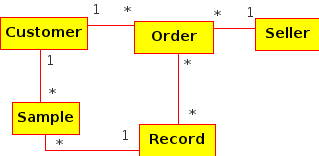
\includegraphics{class_diagram.png}}
    \end{center}
    \caption{Conceptual class diagram}
    \label{fig:class_diag}
\end{figure}
\begin{description}
    \item[]
        The figure shows 4 simple classes and the relations between them.
    \item[]
        Each Customer can make several orders and an order can contain several
        records an order can also contain the same record many times (eg. different vinyl color).
    \item[]
        Each Seller handles several orders.
    \item[]
        Each record can have many samples and each customer can 
        listen to as many samples as he/she likes.
\end{description}

\newpage
\subsection{Activity diagram}
\begin{figure}[htb]
    \begin{center}
        \setlength\fboxsep{0pt}
        \fbox{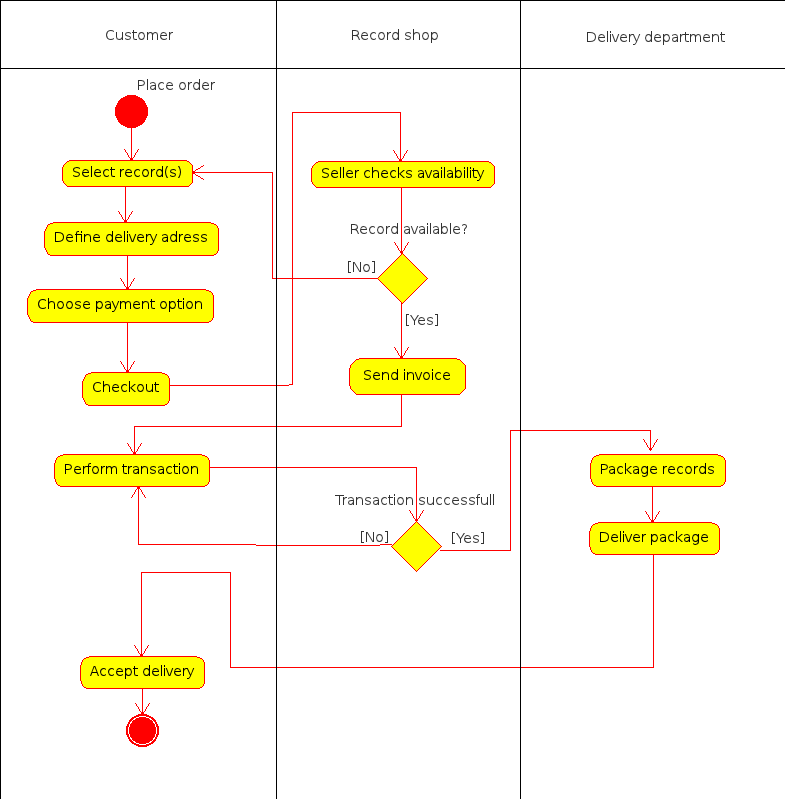
\includegraphics[scale=0.65]{activity_diagram.png}}
        \caption{Activity diagram}
        \label{fig:activ_diag}
    \end{center}
\end{figure}
\begin{description}
    \item[]
        The customer selects the records he/she wishes to order, defines the delivery
        address and selects the payment option and proceeds to the checkout.
    \item[]
        The system contacts a seller which checks if the record is available.
        If the record is available the Seller sends an invoice to the Customer,
        if the record is out of stock the Customer has the option to choose a different
        record or to discard the order.
    \item[]
        After receiving the invoice the Customer performs the transaction.
        If the transaction is successfull the delivery department packages the records,
        delivers them and the Customer accepts the delivery.
\end{description}

\end{document}
